\subsection{Vector representations} \label{unsupervised_approach_representations}

In this section, we talk about the vector representations of the three different elements of our corpus (documents, venues and subjects). This procedure is an adaptation of \acrshort{mag}'s approach \cite{shen2018web} to our scenario. An important difference between our setting and that of \acrshort{mag} is that ours includes theses, which are not published in any venue.

In the following three sections we will look at the information used to represent venues, documents and subjects. Each element has both a \acrfull{srt} and an \acrfull{ert}. The \acrshort{srt} consists of basic information of the element, whereas the extended one comprises information of associated elements, which are used to enrich the representation of each element.

\subsubsection{Venues}

Venues are journals, conferences and other organizations where researchers can publish their work. They usually accept publications regarding a certain field, such as the \textit{Journal of Clinical Medicine}, which publishes medical work. Some are even more specific, such as the \textit{International Conference on Dublin Core and Metadata Applications}, which only includes publications that have to do with metadata, an area of computer science. Others are more interdisciplinary, including publications of different fields. An example of such a venue is the \textit{Journal of Chemical Physics}, which is a subdiscipline of both Chemistry and Physics. There are venues that are even more broad, such as the famous \textit{Nature}, which comprises all natural sciences and technology.

Regardless of their scope, venues can be useful to identify what topics their publications revolve around. Therefore, the representations of venues are used in the representations of documents. Specifically, their representations are added, with the venue's representation being weighted down. The venues present in the repositories were already analyzed in section \ref{repo_analysis_venues}. Given that there are many types of venues, they appear under various names in the repositories, such as \textit{Journal title} or \textit{Proceedings}. How venues are stored also differs between repositories.

An important difference between our use case and \acrshort{mag}'s, is that we also consider theses, which are not published in any venue. We argue that advisors and referees have a similar role for theses as venues have for publications. We therefore use them as a replacement for venues when considering theses. We then look at how \acrshort{mag} computes the \acrshort{ert}s of venues, and how we do so in our use case. In the end, venues are represented by a sample of the documents they are assigned to, whose representations are concatenated.

\paragraph{Alternative venues for theses} \mbox{} \label{unsupervised_approach_venues_theses}

Given that 36 \% of our documents are theses and thus were not published anywhere, we require a workaround that allows for theses to also be grouped by the topics they handle. If we didn't find an alternative, the representations of theses would be considerably less precise than those of publications, which would hamper the quality of the \acrshort{si}. Just as venues publish research work that handles the topics they focus on, referees and advisors of theses only do so when the topics handled by the student aligns with their fields of expertise. They are therefore good indicators of the semantic content of a thesis.

As discussed in section \ref{repo_analysis_contributors}, theses of edoc and refubium almost always have at least one referee (only 1 \% and 5 \% of the theses don't have one, respectively). On the other hand, 19 \% of the theses of depositonce are missing a referee. The missing referees in depositonce are luckily replaced by advisors. Depositonce is the only repository where advisors appear often. Only 4 \% of the theses there don't have one. Edoc and refubium have almost no advisors.

Given the differences among the repositories, both referees and advisors have to be considered as an alternative for venues when grouping theses. When doing so, only 5 documents of depositonce (0.07 \%) don't have an expert (i.e. neither an advisor nor a referee). 30 documents of edoc (0.4 \%) are also missing an expert, as well as 662 documents of refubium (5 \%). These and other facts are shown in table \ref{tab:experts}, including that, on average, theses feature more than two experts. This may help identify the topics of theses that are multidisciplinary, i.e. whose subjects belong to several fields.

\begin{table}[]
    \centering
    \begin{tabular}{|c|c|c|c|c|}
    \hline
         \thead{Repository} & \thead{No. of \\ experts} & \thead{No. of distinct  \\ experts} & \thead{Avg. no. \\ of experts \\ per thesis} & \thead{No. of theses \\ without \\ an expert} \\
         \hline
         depositonce & 8,383 & 2,338 & 2.6 & 5 (0.07 \%) \\
         \hline
         edoc & 7,308 & 3,395 & 2.8 & 30 (0.4 \%) \\
         \hline
         refubium & 9,133 & 4,863 & 2.2 & 662 (5 \%) \\
         \hline
    \end{tabular}
    \caption{Facts regarding the experts of theses.}
    \label{tab:experts}
\end{table}

\paragraph{Simple representation} \mbox{}

\acrshort{mag} uses the name of the publishing venue as its \acrshort{srt} \cite{shen2018web}. For referees and advisors, we could use the name of the person as its \acrshort{srt}. However, the names of professors have no relationship with their fields of expertise, and therefore would not provide any information about the topics they work on. We therefore discard the names of venues altogether, for the sake of simplicity.

\paragraph{Extended representation} \mbox{}

\begin{figure}
    \centering
    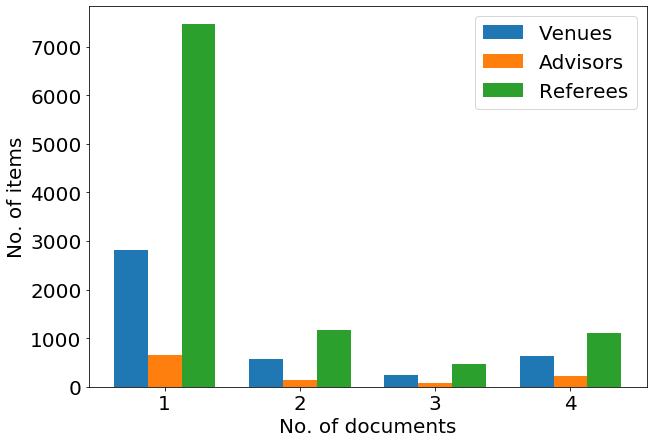
\includegraphics[width=.7\textwidth]{figures/unsupervised_approach/ert_counts.png}
    \caption{No. of documents included in the creation of the ERT of venues, referees and advisors.}
    \label{fig:ert_counts}
\end{figure}

The \acrshort{ert} of a venue is formed by concatenating the \acrshort{srt}s of a sample of its publications. The authors of \acrshort{mag} don't specify how many publications they use for the \acrshort{ert} of each venue. Given that our venues have on average 4.2 publications assigned to them, we pick 4 as the maximum sample size. Venues with less than four documents will take as many documents as there are available to compute their \acrshort{ert}. We do the same for advisors and referees. Those that have more than four documents available are assigned the four longest documents in terms of the number of tokens that are present in the vocabulary, instead of randomly sampling four documents. In this way, we improve their representations by ensuring they comprise as many tokens as possible.

Figure \ref{fig:ert_counts} shows how many documents are used to represent each item (venue, referee or advisor). Most of the items only include one document in their representations. This is the case for 66 \% of the venues, 59 \% of the advisors and 73 \% of the referees. This fact will be important when evaluating the accuracy of our vector representation for the items. Items that include more documents are expected to have more accurate vector representations.

There are six venues and thirteen referees that cannot be represented. Even if they have documents assigned to them, these do not include any tokens that are present in the vocabulary. There are also several more that have only a few tokens on average, as can be seen in figure \ref{fig:bow_venues}. On the other hand, there are only three advisors with less than nine tokens on average. These averages refer to the avg. amount of tokens of their constituent documents, i.e. those that were picked for their \acrshort{ert}.

\begin{figure}
    \centering
    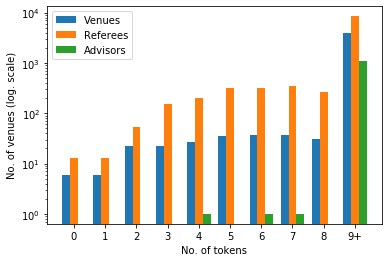
\includegraphics[width=.7\textwidth]{figures/unsupervised_approach/bow_venues.png}
    \caption{Avg. number of tokens of venues, referees and advisors.}
    \label{fig:bow_venues}
\end{figure}

\subsubsection{Documents}

Documents are the publications and theses of the repositories that are written in English. The \acrshort{srt} of a document comprises its title and abstract, and the \acrshort{ert} results from concatenating the \acrshort{ert} of its venue. In this section, we will look at both representations, comparing our implementation with that of \acrshort{mag}. There are some challenges that arise from the small size of our dataset. For instance, the extracted references often pointed to papers outside our dataset, being thus of no use to relate documents to one another.

\paragraph{Simple representation} \mbox{}

Creating the \acrshort{srt} of the documents is straight forward. We can extract the title and the abstract of a document through the OAI-PMH interface of each repository. \acrshort{mag} also uses the keywords, but these are not available in the metadata of the papers. We therefore only use the title and the abstract to represent each document. We cannot use the subjects assigned by the users that uploaded the documents because these will be used to evaluate the performance of our model.

We discard using the full texts of the documents because doing so would complicate the encoding task. Only the most important aspects covered by the paper are included in the abstract, which are the ones we want to consider. Using the full texts could potentially reduce the quality of the encodings, as they cover topics that are not central to the ``aboutness'' of the paper, such as the related work. Furthermore, extracting the texts from the PDFs is time-consuming and computationally expensive.

After processing the texts and removing the tokens that are not included in the vocabulary, documents have on average 37 tokens. 85 documents don't have any, and over 84 \% of them have nine or more tokens. These and some other facts, along with figure \ref{fig:bow_data}, were already discussed in section \ref{vocab_results}, as they were used to determine the size of the vocabulary.

\paragraph{Reference and citation extraction} \mbox{} \label{unsupervised_approach_references}

A reference used by a document $A$ is another document $B$ which the document $A$ uses to lay the foundation of their work. It gives the reader an understanding of the scope of their work, as well as the fields involved. Document $B$ is then cited by document $A$, i.e. citations can be understood as the inverse relations of references: if document $B$ is a reference of document $A$, document $A$ is a citation of document $B$.

To extract the references from the papers, we use a package called \textit{refextract}\footnote{\url{https://github.com/inspirehep/refextract}}. It returns the references it finds in a given text as a dictionary, which includes the title, authors, journal title and other data about each of the referenced papers. Refextract uses regular expressions to identify the elements of the reference, as well as mappings for special cases. It was developed to be used for scientific papers of \textit{High-Energy Physics}\footnote{\url{https://www.energy.gov/science/hep/high-energy-physics}}, an American laboratory. This means that the special cases included in the knowledge bases focus on this specific set of papers. Therefore, we expect the accuracy to be worse in our heterogeneous dataset, which comprises papers written in various formats as well as theses.
 
Using this package, together with a Python port to the Apache Tika library\footnote{\url{https://github.com/chrismattmann/tika-python}} to parse the text from the PDF files, we successfully extracted the references of 29,329 documents. Only 5 documents of depositonce and 14 of refubium didn't have any references. In edoc there are 50 files where no references could be extracted. These documents either did not have any files, the file did not include references, or the format of the references could not be identified.

The documents for which we could extract references, include on average 157 references. This number is so large because of the theses, which on average comprise 246 references. Publications include on average 105 references. This number is so large because of refubium, whose documents include on average 121 references. Edoc and depositonce include 85 and 91 references on average, respectively. Unfortunately, most of these references point to documents outside the repositories. Only 328 documents (1.2 \% of all the documents) refer to other documents in the repositories. They do so an average of six times. The remaining 29,001 documents (99 \% of all documents) cannot be related through their lists of references.

\paragraph{Extended representation} \mbox{}

In \acrshort{mag}, the \acrshort{ert} of a document comprises three different aspects (references, citations and venues). As was just mentioned, the size of our dataset is too small to profit from relations among papers through their lists of references. Therefore, we only use the \acrshort{ert} of its associated venues, referees and advisors. These are added to the \acrshort{srt} after being multiplied with a weighting factor $w$. Here is the equation for computing the \acrshort{ert} of documents:

$$ h_e^d = h_s^d + w \cdot \frac{1}{n} \sum_V h_e^V $$

$h_s^d$ refers to the \acrshort{srt} of a document; $h_e^V$ refers to any venue, advisor or referee that is related to the document. The creators of \acrshort{mag} don't disclose how they weighted venues in the paper. Therefore, we decided to choose $0.7$ as the weight parameter. Our choice is probably higher than the one used in \acrshort{mag}. This makes sense as we have less data available to represent documents.

Once the representations of documents are enriched with the representations of their venues, only 33 documents remain without tokens, out of the 85 that were empty before. The number of tokens per document is illustrated in figure \ref{fig:doc_representations}, which can be compared to figure \ref{fig:bow_data}, where the same data is shown but without including venues. On average, document representations comprise 324 tokens, including tokens of 1.5 venues. 20,399 documents include only one venue, whereas 7,430 documents include either two or three venues. Almost 98 \% of the documents have more than eight tokens in their \acrshort{ert}.

\begin{figure}
    \centering
    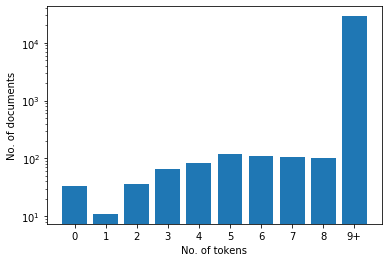
\includegraphics[width=.7\textwidth]{figures/unsupervised_approach/doc_representations.png}
    \caption{Number of tokens in the extended representation of the documents.}
    \label{fig:doc_representations}
\end{figure}

\subsubsection{Subjects}

Subjects are the concepts we use to describe the content of the documents. Each document is assigned a variable number of subjects, which together define what the document is about. We already discussed how subjects were retrieved from OpenAlex in section \ref{problem_scope_subjects}. The resulting set comprises 2,157 subjects, evenly distributed among the 19 fields.

Here, we explain what information we use to describe the subjects. Microsoft performed manual steps to create the \acrshort{ert} of the subjects that we are unable to emulate. Therefore, subjects only comprise a \acrshort{srt}, which is their Wikipedia article. This is the only external information we use throughout this approach, as we have not found any other way to represent subjects.

\paragraph{Simple representation} \mbox{}

Each \acrshort{mag} subject is associated to a Wikidata page, from which we can extract the Wikipedia link. We parse the HTML tree of the Wikipedia pages with the \textit{lxml} package\footnote{See \url{https://github.com/lxml/lxml}}, which allows us to navigate the tree with XPath expressions. We use them to avoid retrieving the texts of quotes, tables, or images, which sometimes appear before the content of the page. Once we arrive at the content, we retrieve paragraphs until we have gathered at least 500 characters.

If there is no link to an English Wikipedia entry, we use the Wikidata description as the \acrshort{srt}. This is the case for only three subjects: \textit{Discretization}, \textit{Statute} and \textit{Interim}. The \acrshort{srt}s of these subjects comprise 71, 40 and 33 characters, respectively. All other subjects have \acrshort{srt}s with more than 500 characters.

On average, the \acrshort{srt}s of the subjects comprise 752 characters. Regarding tokens that are present in the vocabulary, the Wikipedia articles have on average 30 tokens. Only four subjects have less than nine tokens: the three for which no Wikipedia page was found and \textit{Athletes}, whose Wikipedia page really consists of just one sentence.

\paragraph{Extended representation} \mbox{}

The research group of Microsoft manually assigned subjects to venues and used the \acrshort{ert}s of a sample of venues as the \acrshort{ert} of the subject. Doing so is a lot of work, which is out of reach for this thesis, as we don't have the manpower of Microsoft. We therefore only use the Wikipedia articles to represent the subjects.
